% \chapter{模板的安装与使用}
% \label{chp:installation}

% 本章将介绍如何配置 \LaTeX 开发环境并使用本模板编译PDF格式的论文。
% \nomenclature{PDF}{Portable Document Format}

% \section{环境准备}
% \label{sec:tex_environment}

% 使用本模板之前首先需要在你的设备上配置好 \LaTeX 开发环境。目前主流的计算机操作系统都对 \LaTeX 有较好的支持,接下来我们将以几个常见操作系统为例介绍环境的配置方法。

% \subsection{Microsoft Windows\texttrademark}

% \LaTeX 在Microsoft Windows操作系统上的发行版称为 Tex Live,该发行版提供了较为全面的现代 \LaTeX 编译引擎支持,包括了对 XeLaTeX 和 LuaTeX 的良好支持。需要强调的是,一些网络上的教程可能会指导初学者下载 CTeX 安装套件,请不要这样做。CTeX 是刀耕火种时代 \LaTeX 社群针对中文使用者发明的妥协产物,在早期有其使用价值,但现如今在使用时往往会面临宏包缺失和兼容性问题\cite{muzi2020ctex}。为了避免你在issue中反复抱怨编译错误,或者发邮件询问一个本不该出现的问题,请珍爱生命,使用 Tex Live。

% 截止到本文撰写的时间点,Tex Live的最新版本为Tex Live 2019,你可以在\href{http://tug.org/texlive/}{这个网站}找到下载链接。请尽量选择完全下载并本地安装而非使用下载器在线安装,因为大部分中国IP的连接速度让人绝望。下载时你可以就近选择节点,如果你使用的是校园网的话可以达到一个相当可观的下载速度。

% 安装过程较为简单,按照步骤设定安装位置即可。需要注意的是,请你在安装完成后设定好环境变量。尽管不设定环境变量在多数情况下也可以工作,但是你将无法使用我们提供的编译脚本。设定环境变量的方法与步骤不在本文的教程范围之内,请自行百度。

% \subsection{Apple MacOS\texttrademark}

% \LaTeX 在Apple MacOS操作系统上的发行版称为MacTeX。在 MacOS 上安装 MacTeX 之前,请确保你已经正确安装了\href{https://brew.sh/}{homebrew}。当然,你也可以直接从\href{http://www.tug.org/mactex/index.html}{官网}下载 MacTeX套件,但本文建议你使用 homebrew 安装纯净的 MacTeX 发行版。MacTeX 分为基本版和完全版,区别主要在于完全版中默认包含了更多的宏包。安装基本版 MacTeX 已经可以应付你绝大多数 \LaTeX 需求,在终端中输入:

% \begin{tcolorbox}
% \begin{lstlisting}
% brew cask install basictex
% \end{lstlisting}
% \end{tcolorbox}

% \noindent 你就可以获得了基本版的 MacTeX。如果你一定要安装完全版,请在终端中输入:

% \begin{tcolorbox}
% \begin{lstlisting}
% brew cask install mactex
% \end{lstlisting}
% \end{tcolorbox}

% \subsection{Ubuntu Linux}

% 在 Ubuntu 中配置 \LaTeX 开发环境最为简单。事实上如果你是一个 GNU/Linux 使用者,你应该已经具有了相当的工程能力能够自行配置 \LaTeX 编译环境。但为了本文结构上的完整,我们决定还是多此一笔。在终端中输入:

% \begin{tcolorbox}
% \begin{lstlisting}
% sudo apt install texlive-full
% \end{lstlisting}
% \end{tcolorbox}

% \noindent 你就可以在 Ubuntu 设备上部署 Tex Live 发行版。其他 Linux 发行版上的安装方法与 Ubuntu Linux 类似,只是各自使用的包管理器可能有所不同,请参阅各发行版的包管理中心网站,本文不再赘述。

% \section{模板的下载与安装}
% \label{sec:template_download}

% 其实在你看到本手册的同时,我们相信你已经成功地将本模版下载到了你的设备上。因此本来并没有必要在此赘述介绍工程的下载方法。但为了防止你下载的并非最新版本的模板工程,或者本模板被其他网站转载而你恰好从别的网站上下载了本模板,我们觉得还是有必要介绍一下我们指定的下载地址。本模板工程的所有代码都已经在GitHub上开源,你可以从\href{https://github.com/herculas/SEU-master-thesis}{这个地址}找到本模板的最新版本。

% 将本模板工程文件解压缩到你喜欢的目录下,你就得到了完整的模板工程。为了避免不必要的编译问题,我们建议你将工程保存在全英文的目录下。本模板已在 Windows 10,MacOS 10.15 Catalina,Ubuntu 18.04 Bionic Beaver以及Manjaro 19.0.2 上编译通过,但需要注意的是一些 Linux 发行版中没有安装本模板编译所需的字体文件,如宋体、黑体、楷体和 Times New Roman 等。因此如果你在 Linux 下遭遇了编译问题,请首先检查你的字体是否都已经安装完好。

% \section{论文的编译}
% \label{sec:compilation}

% 如果你使用的是如 Tex Studio,Texpad 或 WinEdt 等 \LaTeX 集成环境,你可以从这些软件中直接启动编译。但是作为一个较为庞大的、涉及多文件的 \LaTeX 工程,你可能需要多次编译才能获得完整的论文。一个完整的编译过程包含下面几个步骤:

% \begin{tcolorbox}
% \begin{lstlisting}
% xelatex main
% bibtex main
% makeindex main.nlo -s nomencl.ist -o main.nls
% xelatex main
% xelatex main
% \end{lstlisting}
% \end{tcolorbox}

% \noindent 想要编译一篇学位论文,首先需要对文章结构和原始文本进行一次预编译;随后索引出论文中出现的所有参考文献,并建立参考文献条目与论文引用位置的连接;接下来,根据预编译所产生的文章结构,需要生成文章的图表和术语索引文件;最后通过两次编译将参考文献和图表索引编入正文中,得到完整的PDF版本论文。可以看到这个过程极其复杂,因此我们为你准备了两个脚本文件,来将你从复杂的编译流程中解脱出来。对于 Windows 用户,你可以双击工程根目录下的 make.bat 文件启动编译流程。而 MacOS 和 Linux 用户则可以在命令行中执行根目录下的 make.sh 脚本来启动编译流程。

\chapter{绪论}
\section{研究背景和意义}

无线通信在民事和军事应用中已经发挥着不可替代的作用,研究无线通信的安全性具有重要研究价值。无线网络由于接入层的开放性,因此容易遭受攻击。无线网络的安全性通常由传统密码学保证,比如公钥基础设施(PKI)。PKI被广泛应用于保护计算机网络,但在很多轻量级的无线通信系统中,如物联网系统中的应用受到了限制。由于PKI是依赖高时间复杂度算法,而无线物联网设备通常是低功耗设备,对算法的复杂性要求较高。此外,PKI算法的安全性是由数学问题的复杂度决定的,比如大整数分解问题等,随着量子计算的发展,此类问题在未来将有被攻破的风险。

\subsection{当前无线通信网络中存在的问题}

由于无线通信系统的开发性,无线通信中的信息传输可能遭到窃听、篡改和伪造。为了保护信息的完整、可信,需要在无线网络中需要建立针对每一次通信加密用的会话密钥。

然而,无线通信网络的开放性、脆弱性和拓扑性,使得无线通信网络极易遭受攻击:

1. 相对于有线网络,由于物理边界的缺失,无线通信网络的广播特性使得范围内任意用户可以接入网络,使得传输信息容易被非法用户窃听,并且难以察觉窃听者的地点。
2. 无线通信网络拓扑具有灵活性和移动性,传统的密钥分发方案并不适用于动态变化的网络拓扑结构,在资源受限的节点网络中,影响更为突出。

另外,传统的安全机制主要通过上层协议(应用层、传输层)的加密来实现,传统安全通信需要第三方机构注册证书、分发密钥,然后通过会话密钥进行会话。传统安全通信是“有条件”的安全,因为其安全性是建立在非法用户的计算能力有限的基础上,随着算力提高和硬件发展,密码学相关算法或被攻破。传统安全通信即使保证上层协议的安全,也无法完全避免物理层的恶意干扰,因此物理层安全的相关研究应运而生,出现了大量物理层的安全机制相关的研究。

物理层安全机制可以从根本上解决无线通信的安全性问题,与传统安全机制相比,物理层安全从物理层实现信息的安全处理。在物理层安全机制的研究工作中,基于密钥的物理层安全机制将传统安全机制和物理层安全机制相结合的方案,具有高可行性和高可靠性的特点,其特点是通过无线信道的特性进行密钥生成的相关工作,最后提供密钥给上层应用直接使用。

\subsection{无线信道密钥生成技术}

无线信道密钥生成技术属于物理层安全的范畴,通过利用合法通信双方之间的信道特性,估计无线信道特征,量化生成会话密钥,进而将会话密钥提供给上层协议使用。

物理层安全不同于传统密码学,目前演化成了两个分支,无密钥安全和基于密钥的安全机制。其中无密钥实现复杂,需要苛刻的信道条件。公共信道上的无条件密钥安全由Bennett、Brassard和Robert提出\cite{bennett1985reduce}\cite{bennett1988privacy}。Ahlswede和Csiszar等人进一步泛化和改善\cite{ahlswede1993common}。Maurer等人建立了一个通用的信息论模型\cite{maurer1993secret}。基于密钥的安全机制是将物理层安全和传统安全机制结合的安全方案。在无线通信网络中,无线信道通信的特性有以下特性:

\begin{itemize}
    \item \textbf{短时互易性}。在时分双工(Time Division Duplex, TDD)系统中,通信双方的上下行信道在相干时间内具有相似的信道特征。
    \item \textbf{随机性}。随着时间变化,周围环境中物体的移动会扰动信道,造成信道随机变化,通过信道特征提取的密钥自然也具有随机性,因此每次协商的密钥都将不可预测,这符合安全机制对密钥的要求。
    \item \textbf{地理空间位置唯一性}。无线信号的传输是开放的,因此将不可避免的会有窃听者存在。然而,无线信道的多径衰落对位置信息敏感。当窃听者距离合法通信者在无线通信电磁波频率半波长范围外,其无线信道的多径衰落不同,因此其窃听测量得到的信道特征也和合法通信者不相关,从而无法获得真正的密钥。
\end{itemize}

由于无线通信信道具有上述特性,因此在物理层协商生成安全、可靠的密钥是可行的,一方面不依赖第三方传输机构,另一方面计算复杂度较小。

\section{国内外研究现状}

无线通信的广播特性允许范围内其他用户接收信号,因此容易遭受攻击。攻击者可以利用该特性进行被动攻击,比如窃听和监控信息、分析网路流量,或者进行主动攻击,比如修改消息、伪造认证、重放攻击以及拒绝服务(Dos)攻击\cite{Zhang2016Key}。传统的安全工作依赖于公钥算法体系,比如RSA等算法,因为窃听者破译信息所需时长远远超过信息本身的价值,由此保障后向安全。

图\ref{wirelss-network-security}所示传统加密方法包含对称加密和非对称个加密,对称加密算法使用相同的一对密钥,可以用于对加密时间要求较高的场景;非对称加密算法使用一对公钥和私钥,通常用于密钥分发。

传统加密算法有以下几个问题。首先,传统加密算法依赖一些数学问题的计算难度,比如离散对数问题\cite{forouzan2007cryptography}。随着硬件发展和算力的大幅提升,通过计算难度保证安全不再可取。此外,传统加密算法需要一个可信的密钥管理设施,并不适用于去中心化的无线传感器网络(WSN)和无线自组网络,并且传感器节点的计算能力有限。

即使通信协议的上层应用了传统加密算法,也需要从物理层层面加强通信安全以抵抗攻击。物理层安全(PLS)可以利用无线信道的不可预测性和随机性来达到信息论安全。如图\ref{wirelss-network-security}所示,PLS方法包括无密钥安全和基于密钥的安全机制。在Wyner\cite{wyner1975wire}和Csiszar{csiszar1978broadcast}等人提出的窃听信道模型中,无密钥安全不需要加密密钥,而是通过合法用户和窃听者之间不同的信道特性来保证安全\cite{6739367},,当合法通信信道优于窃听者信道时,合法通信双方之间便可以协商出安全的密钥。文献\citen{peng2017secret}提到,即使窃听者信道由于合法通信信道,也存在方法来协商出安全的密钥。比如,文献\citen{parada2005secrecy}、\citen{liu2009note}和\citen{li2007secret2}分析了慢衰落信道\cite{gopala2008secrecy}、快衰落信道\cite{li2007secret}以及多天线条件下密钥容量。合法用户需要知道第三方窃听者的瞬态或者稳态信道状态信息(CSI),但是在生产环境中,获取第三方窃听者的瞬态和稳态信号比较复杂、不易实现。

基于密钥的安全机制追随到1919年提出的Vernam加密,即一次一密\cite{vernam1922secret}。之后,香农为完全保密提出理论基础\cite{shannon1949communication}。当密钥Key的信息大于等于消息M的信息时,消息M可以被编码成码字C,并不会泄露任何消息,即

\begin{equation}
    H(M|C) = H(M)
\end{equation}

其中,$H(\cdot)$表示熵。然而,在生产环境中,在合法用户之间协商不可重用的随机密钥是非常困难的。一种可行的方案是,将密钥生成和对称加密结合在一起形成混合加密系统。

\begin{figure}[htbp!]
    \centering 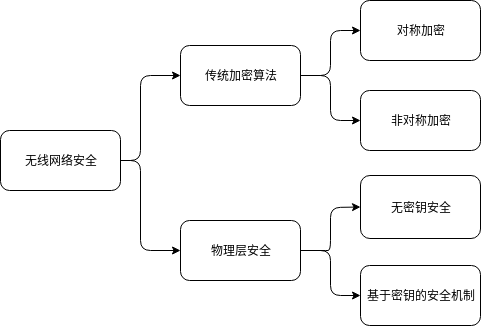
\includegraphics[width=0.6\textwidth]{images/wireless-network-security} 
    \caption{无线网络安全}
    \label{wirelss-network-security}
\end{figure}

本文研究无线信道密钥生成,即利用无线信道的随机性来生成密钥。和公钥体系利用数论问题保证安全性不同,无线密钥生成的安全性基于信息论。因为它基于无线信道的随机性\cite{ahlswede1993common}\cite{maurer1993secret},并且不需要借助其他用户的信息。以上所提及方法的优缺点列在表\ref{comparison-different-schemes}。

\begin{table}[]
    \centering
    \begin{tabular}{|p{80pt}|p{90pt}|p{70pt}|p{90pt}|p{90pt}|}
    % \begin{tabular}{|l|l|l|l|l|}
    \hline
    方法 & 描述 & 实现复杂度 & 优点 & 缺点 \\ \hline
    对称加密 & 合法通信双方用对称密钥加密数据 & 易实现 & 算法复杂度低 & 提前协商会话密钥;计算安全性 \\ \hline
    非对称加密 & 合法通信双方使用一对公私钥协商会话密钥 & 易实现 & 可用于协商会话密钥 & 计算安全性;依赖PKI;不适于低功耗设备 \\ \hline
    无密钥安全 & 合法通信双方通过设计编码和信道特性避免泄露信息 & 实现复杂 & 信息论安全;无需密钥的安全传输 & 依赖窃听者的CSI \\ \hline
    基于密钥的安全机制 & 合法通信双方利用信道的随机性生成密钥 & 易实现 & 信息论安全;轻量;无需第三方参与 & 受限于信道特性本身 \\ \hline
    \end{tabular}

    \caption{不同方法的比较
    \label{comparison-different-schemes}}
\end{table}

物理层安全的一个重点研究方面是密钥生成(SKG,Secret Key Generation)。1993年Maurer和Ahlswede等人理论上提出密钥生成\cite{ahlswede1993common}\cite{maurer1993secret},研究一对观察共用随机源的合法通信者之间的密钥生成速率,并且该随机源对第三方窃听者透明。对于TDD模式的无线通信网络来说,由于上下行信道之间的短时互易性,合法通信双方可以使用无线信道衰落特性作为密钥生成的随机源。密钥生成的信道模型如图\ref{wireless-channel}所示。图\ref{wireless-channel}中Alice和Bob需要建立一个安全的加密通道,窃听者Eve与Alice相距d厘米,并监听了所有传输过程。Alice、Bob和Eve可以分别接收到信号$X^n = (X_1, ..., X_n)$,$Y^n = (Y_1, ..., Y_n), Z^n = (Z1, ..., Z_n)$。Alice和Bob在公共信道上交换消息s,Eve同样可以接收到消息s。对任何$\epsilon > 0$和足够大的$n$,如果存在$K^A = g_A(X^n, s)$和$K^B = g_B(Y^n, s)$使得密钥生成体系满足

\begin{eqnarray}
    Pr(K^A \neq K^B) < \epsilon \label{keyrate1} \\
    \frac{1}{n}I(K^A; s, Z^n) < \epsilon \label{keyrate2} \\
    \frac{1}{n}H(K^A) > R - \epsilon \label{keyrate3} \\
    \frac{1}{n}log[\mathcal{K}] < \frac{1}{n}H(K^A) + \epsilon \label{keyrate4}
\end{eqnarray}

那么式中R即可达密钥速率,其中$I(\cdot)$表示互信息,$\mathcal{K}$表示密钥key的字母表。公式(\ref{keyrate1})表示Alice和Bob生成相同密钥的可能性;公式(\ref{keyrate2})表示通过公共信道传输消息,不会泄露给窃听者Eve,从而保证密钥安全性;公式(\ref{keyrate4})确保密钥是均匀分布。最大可达密钥速率可以用密钥容量定义,

\begin{equation}
    C_K = min[I(X;Y), I(X, Y|Z)]
\end{equation}

在具有丰富多径的无线通信环境中,信道响应具有空间唯一性,因此当上下行链路与上下行链路之间的距离超过半个波长,所有的上下行链路的信道响应之间是互相独立的\cite{jakes1994microwave}。所以第三方窃听者在半波长距离以外,难以分析出与合法通信信道完全精确的信道信息,其构成了基于信道随机性的无线信道密钥生成技术的基石\cite{aono2005wireless, badawy2015secret, koorapaty2000secure, sayeed2008secure, chorti2012helping, shehadeh2012towards, jana2009effectiveness, mathur2008radio, patwari2009high, croft2010robust, liu2014group, azimi2007robust, tope2001unconditionally, liu2014secret, badawy2016robust, zhang2016efficient, xi2014keep, liu2012exploiting, ye2010information, gungor2011secret}。根据密钥生成使用的信道特性,可以将目前研究分为三类,即空间角度\cite{aono2005wireless}\cite{badawy2015secret}、相位
\cite{koorapaty2000secure, sayeed2008secure, chorti2012helping, shehadeh2012towards}和幅度三种。由于离开角和到达角不同,角度的特征通常不互易,因此角度特征不够实用。基于幅度的密钥生成使用的信道特性有接收信号强度(Received Signal Strength,RSS)\cite{jana2009effectiveness, mathur2008radio, patwari2009high, croft2010robust, liu2014group}、信号包络\cite{azimi2007robust, tope2001unconditionally, liu2014secret, badawy2016robust, zhang2016efficient, xi2014keep, liu2012exploiting},幅度交叉
率(Level-Crossing Rate,LCR)\cite{ye2010information}和距离\cite{gungor2011secret}。因此基于相位和幅度的密钥生成方法更加值得研究和关注。

目前已经有一些研究工作实现上述理论。1995年第一个实际的密钥生成协议被提出\cite{hershey1995unconventional},之后陆续出现大量研究无线密钥生成的相关工作。文献\citen{WangSurvey}的第四章从信息论角度阐述了无线密钥生成。文献\citen{WangSurvey}将信道探测和量化合并为一个步骤来研究。文献\citen{zeng2015physical}介绍了密钥生成技术存在的机遇和挑战,但是未涉及到具体实现细节。文献\citen{ren2011secret}总结了一些密钥生成方法,比如基于接收信号强度(RSS)\cite{luo2016rss}和基于信道相位的方法\cite{wang2011fast}。

\section{研究内容和方法}

无线信道密钥生成协议通常包含四个步骤,信道探测、特征量化、信息调和以及隐私放大:

\begin{itemize}
    \item \textbf{信道探测}。信道探测是测量无线信道并提取无线信道特征的过程。通信双方互相收发导频信号,并从接收到的导频信号中提取信道特征。
    \item \textbf{特征量化}。特征量化是将无线信道特征通过预处理、归一化、量化等操作得到比特流的过程。由于提取的无线信道特征受到接收端增益等参数的影响,所以需要预处理、归一化等操作来使得双方探测的信道特征更加相近。之后,再量化成比特流。
    \item \textbf{信息调和}。信息调和是利用无线信道特征作为随机密钥源并结合合理可靠的交互协议生成会话密钥的过程。通信双方在探测信道之后,量化信道得到密钥,通过公共信道的交互协议去除密钥中的不一致比特,得到完全一致的会话密钥\cite{cachin1997linking}。
    \item \textbf{隐私放大}。隐私放大是进一步提高密钥随机性和可靠性、去除密钥中信道相关信息的过程。通过单向哈希函数等方法,可以移除密钥中隐藏的信道信息,进一步提高密钥的安全性\cite{cachin1997linking}。
\end{itemize}

本文基于GNURadio软件无线电开发平台,实现一种TDD/FDD下低时延宽带无线信道密钥生成系统。本文系统信道探测部分分为两种模式,一种TDD模式,另一种FDD模式,并研究两种模式下的信道互易性、密钥安全性等,设计TDD模式和FDD模式下低时延的会话密钥协商技术。无论是TDD还是FDD,其核心都是通信双方在相干时间内获取对端发射的导频信号,并从接收的导频信号中分析和提取信道特征。两种模式除了信道探测部分不同,其余三部分均比较相似。

TDD模式和FDD模式的主要不同点是收发导频信号的机制不同。TDD模式下,通信双方工作在同一频率,相干时间内,两个发送端发射的电磁波经管相同的信道衰落;FDD模型下通信双方工作在不同频率,收发导频信号几乎发生在同时。由于合法通信双方的通信信道在空间上唯一性,所以即便第三方窃听者监听到任意一方发送的导频信号,也无法分析出通信双方之间的CSI信息,以此保障密钥的安全。

无论是TDD模式还是FDD模式,通信双方提取出CSI之后的主要过程是相似的:量化、调和。由于无线信道的短时互易性,通信双方的CSI是相近的,在量化之后得到的比特流也是相似的,但是由于信道在探测时隙内发生变化以及周围环境中的干扰等各种因素,双方提取的密钥又是不完全一致的。因此需要进一步调和,去除不一致比特或者纠正错误比特。调和之后,通信双方会获取一致的比特流,为了进一步去除比特流中的信道信息,进行隐私放大得到最终的会话密钥。

本文使用均匀量化的方式处理CSI浮点数数据,先将数据归一化到[0, 1]范围内,再根据量化阶数伸缩数据范围,然后直接向下取整。量化阶数越高,密钥一致率越低;量化阶数越低,密钥一致率越高。量化之后,使用格雷码进一步降低密钥不一致率,再利用8b-10b编码让01比特分布更加均匀、随机。

本文在调和步骤设计了两种调和方式:CRC校验和原始密钥比特流调和。对于前者,本文将量化之后的比特流分组,并生成CRC校验码,根据校验码去除不一致的分组,保证调和之后完全一致的密钥流。对于后者,本文利用纠错码的纠错特性,直接将比特流和消息异或,再进行纠错编码,接收端对接收到的加密消息进行纠错解码,恢复原始消息。

GNURadio是软件无线电开发平台,被广泛应用于音频处理、移动通信、卫星追踪、GSM网络等计算机软件\cite{Blossom2004GNU},用户可以在GNURadio平台上设计、仿真以及部署高性能无线电的软件无线电系统。本文基于GNURadio软件无线电开发平台和USRP N210硬件,设计TDD/FDD下低时延宽带无线信道密钥生成系统,并验证生产环境下无线密钥生成技术的可靠性和安全性。

在现有关于无线密钥生成技术的研究中,无线密钥生成技术的理论和仿真居多,在实际生产环境中实现并验证的研究并不多见。本文基于GNURadio软件无线电平台,设计和开发了TDD/FDD模式下低延迟无线密钥生成系统,并在不同场景下采集数据,通过分析CSI的相关性、信道随机性、密钥随机性、信息泄露率等四种指标,充分验证无线密钥生成技术在实际环境中使用的安全性和可靠性。

\section{本文主要内容与章节安排}

本文主要研究无线信道密钥生成技术及其实际应用。文章先介绍了无线信道密钥生成技术的研究背景,并概述国内外无线信道密钥生成技术的研究现状,在现有研究基础上,基于GNURadio软件无线电平台,设计和开发TDD/FDD模式下低延迟无线密钥生成系统,并提出相应的系统性能评估指标,在多种场景下评估系统性能并分析系统优缺点。

\subsection{本文主要内容}

本文完成的主要工作包括:

\begin{itemize}
    \item(1)分析无线密钥生成技术的意义和背景,介绍无线密钥生成技术的国内外研究现状以及相关问题。
    \item(2)基于无线密钥生成技术的理论,设计完整的无线密钥生成技术方案,搭建TDD/FDD无线密钥生成系统。
    \item(3)基于TDD/FDD无线密钥生成系统,研究不同场景下无线密钥生成系统的安全性和可靠性,通过多次实验分析通信参与者CSI的相关性、无线信道随机性、密钥的随机程度、信息泄露量、密钥生成速率、系统的纠错性能,支撑无线密钥生成技术的实际应用意义。
\end{itemize}

\subsection{本文章节安排}

根据以上研究内容,本文分为六章,具体章节安排如下:

第一章分析当前无线通信网络中存在的问题,介绍无线密钥生成技术的应用背景和需求,概述当前国内外关于物理层安全的研究,最后给出本文研究内容和章节安排。

第二章阐述无线密钥生成系统的理论基础。首先介绍无线密钥生成技术的信道模型以及无线信道特性,之后详细介绍了无线密钥生成技术的主要步骤,最后给出无线密钥生成系统性能指标的理论依据。

第三章详细介绍了无线密钥生成系统的核心部分。首先介绍了系统中使用的导频信号格式以及检测方法,之后详细描述了导频信号收发机的设计方案以及每个组成模块。

第四章基于导频信号收发机设计完整的无线密钥生成系统,分别介绍了无线密钥生成系统的每个运行阶段。描述围绕导频信号收发机设计的时序逻辑,给出本文估计信道、量化特征、信息调和、隐私放大的具体算法。

第五章基于无线密钥生成系统,在实际环境中连续长时间采集数据,通过这些数据计算性能指标,评估不同场景下无线密钥生成系统的性能,比较TDD模式和FDD模式下性能指标的不同。

第六章总结本文主要工作,提出本文研究方法不足之处。